
\documentclass[runningheads]{llncs}
\usepackage[section]{placeins}

\usepackage{hyperref}
\usepackage{graphicx}
\usepackage{booktabs}
\hypersetup{
    colorlinks=true,
    linkcolor=blue,
    filecolor=magenta,      
    urlcolor=cyan,
    pdftitle={Overleaf Example},
    pdfpagemode=FullScreen,
    }
\begin{document}

\title{COMP3330 Assignment1}
\author{Sebastian Hadley}
\institute{University Of Newcastle}
\maketitle

\begin{abstract}
In this report, we assess the effectiveness of different methods of solving Machine Learning problems by solving a selection of problems with different methods and judging how different factors can impact the performance of the solutions.
\end{abstract}
\section{Question 1}

The 2 spiral-problem is quite difficult as it is a relatively small dataset with complex relations that determine the way each data point is classified, because of this it is difficult to build a Neural Network complex enough to identify the correct decision boundaries while also not over-fitting to the training data.
 
\subsection{Part a}

 For the "original dataset" of Lang and Witbrock (1988), different feed-forward Neural Network architectures were experimented with, including varying the number of layers, neurons per layer,learning rate and activation functions. The performance was evaluated on  the different configurations using 10-fold cross validation with each fold being broken up into test and training sets to ensure ability to generalize was being assessed. The quantitative metrics that were judged were, loss and accuracy as well as a qualitative analysis of the decision boundaries. The decision boundaries were output for each fold, as well as a final decision boundary that took the mode class predicted for each point within the grid over all the decision boundaries to output an average decision boundary over the 10-folds.

In the initial attempt the model was constructed with 2 hidden layers each containing 8 neurons, that used the Relu activation function with the output layer using SoftMax. This model was initially tested with a learning rate of 0.01 over 100 epochs, with a few attempts at adjusting the hyper-parameters to tune the results, this architecture performed fairly poorly for all the different hyper parameters that were attempted. \hyperref[tab:1A2LayerResults]{Table~\ref*{tab:1A2LayerResults}} shows the results of a few attempted hyper parameters.

The most successful of these quantitatively is likely the 8 neuron, 100 epoch version, however the version that used 1000 epochs had a promising average decision boundary, that seemed to resemble a spiral.

\begin{figure}[!htb]
  \centering
  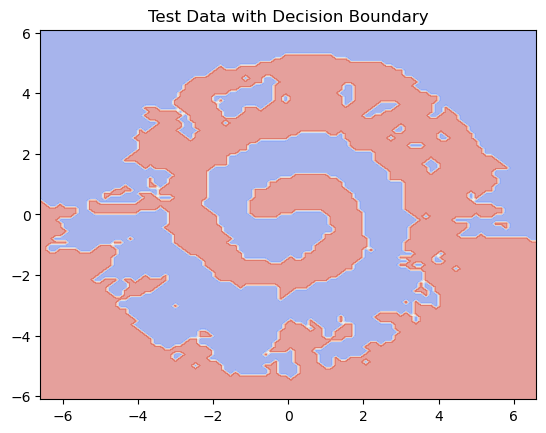
\includegraphics[width=0.5\textwidth]{Question1Images/firstFFNNOutput.png}
  \caption{Average Decision Boundary over 10 folds}
  \label{fig:db}
\end{figure}
\FloatBarrier

These results indicated that despite the small dataset, the relationship between the points is complex enough that we would need to additional layers and neurons. After experimenting with different options, the most consistent results were achieved by a model containing 5 hidden layers aswell as the hyper parameters shown \hyperref[tab:1AFinalModelArchitecture]{Table~\ref*{tab:1AFinalModelArchitecture}} 

\subsection{Part b}

Text for Part b.

\subsection{Part c}

Text for Part c.

\section{Question 2}

\subsection{Part a}

Text for Part a.

\subsection{Part b}

Text for Part b.

\section{Conclusion}

Conclusion text.

\pagebreak
\appendix
\section{Appendix}

\subsection{Question 1}

\renewcommand{\thetable}{1.1}
\begin{table}[ht]
  \centering
  \caption{Results of 2 Layer Architectures}
  \begin{tabular}{c c c c c}
    \toprule
    Epochs \quad & Hidden Neurons \quad & Learning Rate \quad & Average Test Loss \quad & Average Test Accuracy \\
    \midrule
    100 & 8  & 0.01 & 0.84 & 0.38 \\
    300 & 16  & 0.02 & 1.61 & 0.37 \\
    1000 & 16  & 0.02 & 4.91 & 0.42 \\
    \bottomrule
  \end{tabular}
  \label{tab:1A2LayerResults}
\end{table}

\begin{table}[ht]
  \centering
  \caption{Final Model Architecture}
  \begin{tabular}{c c c}
    \toprule
    Epochs \quad & Hidden Neurons \quad & Learning Rate
    \midrule
    1000 & 64  & 0.01 \\
    \bottomrule
  \end{tabular}
  \label{tab:1AFinalModelArchitecture}
\end{table}
%
%\begin{table}[ht]
%  \centering
%  \caption{Results of FAKE FAKE}
%  \begin{tabular}{c c c}
%    \toprule
%    Learning Rate & Loss & Accuracy \\
%    \midrule
%    0.01 & 0.103 & 0.963 \\
%    0.001 & 0.076 & 0.972 \\
%    0.0001 & 0.066 & 0.978 \\
%    \bottomrule
%  \end{tabular}
%  \label{tab:exp2}
%\end{table}




%\begin{figure}[ht]
%\centering
%\includegraphics[width=0.5\textwidth]{loss.png}
%\caption{Training and validation loss over 100 epochs}
%\label{fig:loss}
%\end{figure}

Figures and tables that were placed into the appendix.

\end{document}
